% begin module cylindrical-shells-def
\begin{frame}
\begin{tabular}{cc}
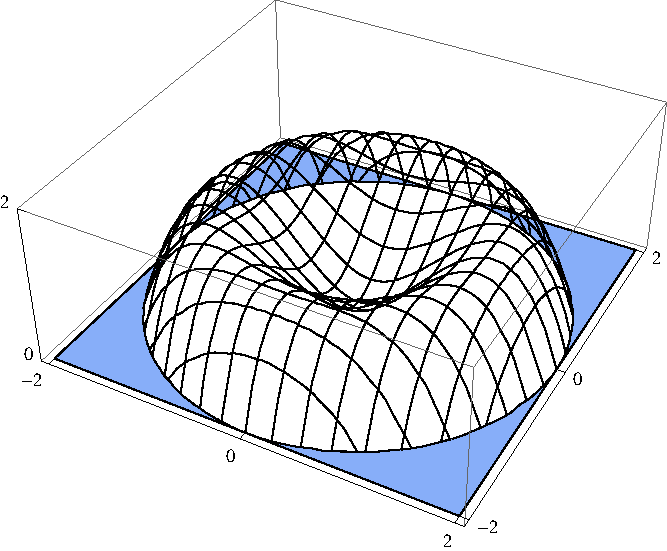
\includegraphics[height=4cm]{volumes/pictures/06-03-setup3d.pdf}%
&%
\uncover<2->{%
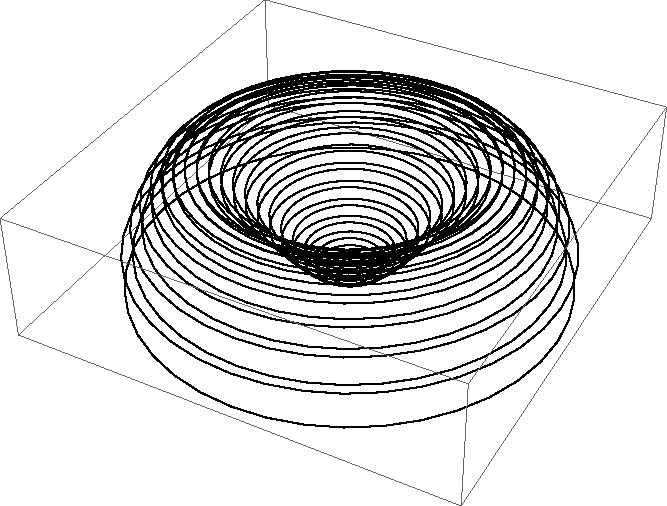
\includegraphics[height=4cm]{volumes/pictures/06-03-setupcylinders.pdf}%
}%
\end{tabular}
\begin{itemize}
\item<1->  Consider the solid obtained by rotating around the $y$-axis the region bounded above by $y = 2x^2 - x^3$ and below by the $x$-axis.
\item<2->  Approximate this solid by nested cylindrical shells.
\item<3->  Cylindrical shells are solids obtained by taking a cylinder and removing from its center another cylinder of equal height but smaller radius.
\end{itemize}
\end{frame}

\begin{frame}
\begin{tabular}{p{3cm}p{7cm}}
\ 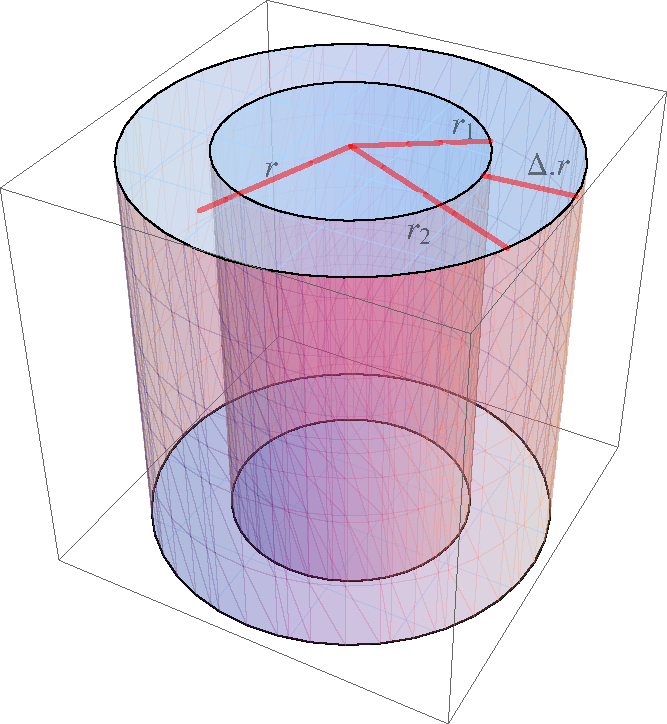
\includegraphics[height=4cm]{volumes/pictures/06-03-cylinder.pdf}%
&%
\begin{itemize}
\item<1->  Consider a cylindrical shell with:
\item<2->  outer radius $r_2$.
\item<2->  inner radius $r_1$.
\item<2->  height $h$.
\item<3->  $V = \pi r_2^2 h - \pi r_1^2 h \uncover<4->{ = \pi (r_2 - r_1)(r_2 + r_1)h}$.
\item<5->  Let $\Delta r = r_2 - r_1$.
\item<5->  Let $r = \frac{r_2+r_1}{2}$.
\item<6->  Then $V = 2\pi rh\Delta r$.
\end{itemize}
\end{tabular}
\end{frame}


\begin{frame}
\[
V = 2\pi rh\Delta r.
\]
\uncover<2->{
If we are approximating the solid obtained by rotating the region under $f(x)$, let the height $h = f(r)$.  Then
\[
V = 2\pi rf(r)\Delta r .
\]
}
\uncover<3->{
If there are $n$ cyclindrical shells $C_1, \ldots , C_n$, let $x_1, \ldots , x_n$ be their radii.  Then
\[
\sum_{i=1}^n 2\pi x_i f(x_i)\Delta x
\]
is the volume of the approximating cylinders.
}

\uncover<4->{
Taking the limit as the number of shells goes to $\infty$, we get
\[
V = \lim_{n\rightarrow\infty} \sum_{i=1}^n 2\pi x_i f(x_i)\Delta x = \int_{\uncover<5->{\alert<handout:0| 5>{a}}}^{\uncover<5->{\alert<handout:0| 5>{b}}}2\pi xf(x) \diff x .
\]
\uncover<5->{
If we are considering the region bounded by $f(x)$ between $a$ and $b$, this gives us the endpoints.
}
}
\end{frame}

\begin{frame}
\begin{definition}[Volume by Cylindrical Shells]
The volume of the solid obtained by rotating around the $y$-axis the region under the curve $y = f(x)$ from $a$ to $b$ is
\[
V = \int_a^b 2\pi xf(x)\diff x .
\]
\end{definition}
\end{frame}
% end module cylindrical-shells-def
